\chapter{Desarrollo del dashboard analítico}
\label{chap:desarrollo_dashboard}

\lettrine{L}{a} capa de presentación es una aplicación web que consume el Datamart de forma segura. La solución se ha desplegado en tres contenedores Docker interconectados: un backend FastAPI (API REST), un frontend React y un proxy inverso Nginx que actúa como único punto de entrada (Figura~\ref{fig:diagrama_nginx_deploy}).

\begin{figure}[htbp]
    \centering
    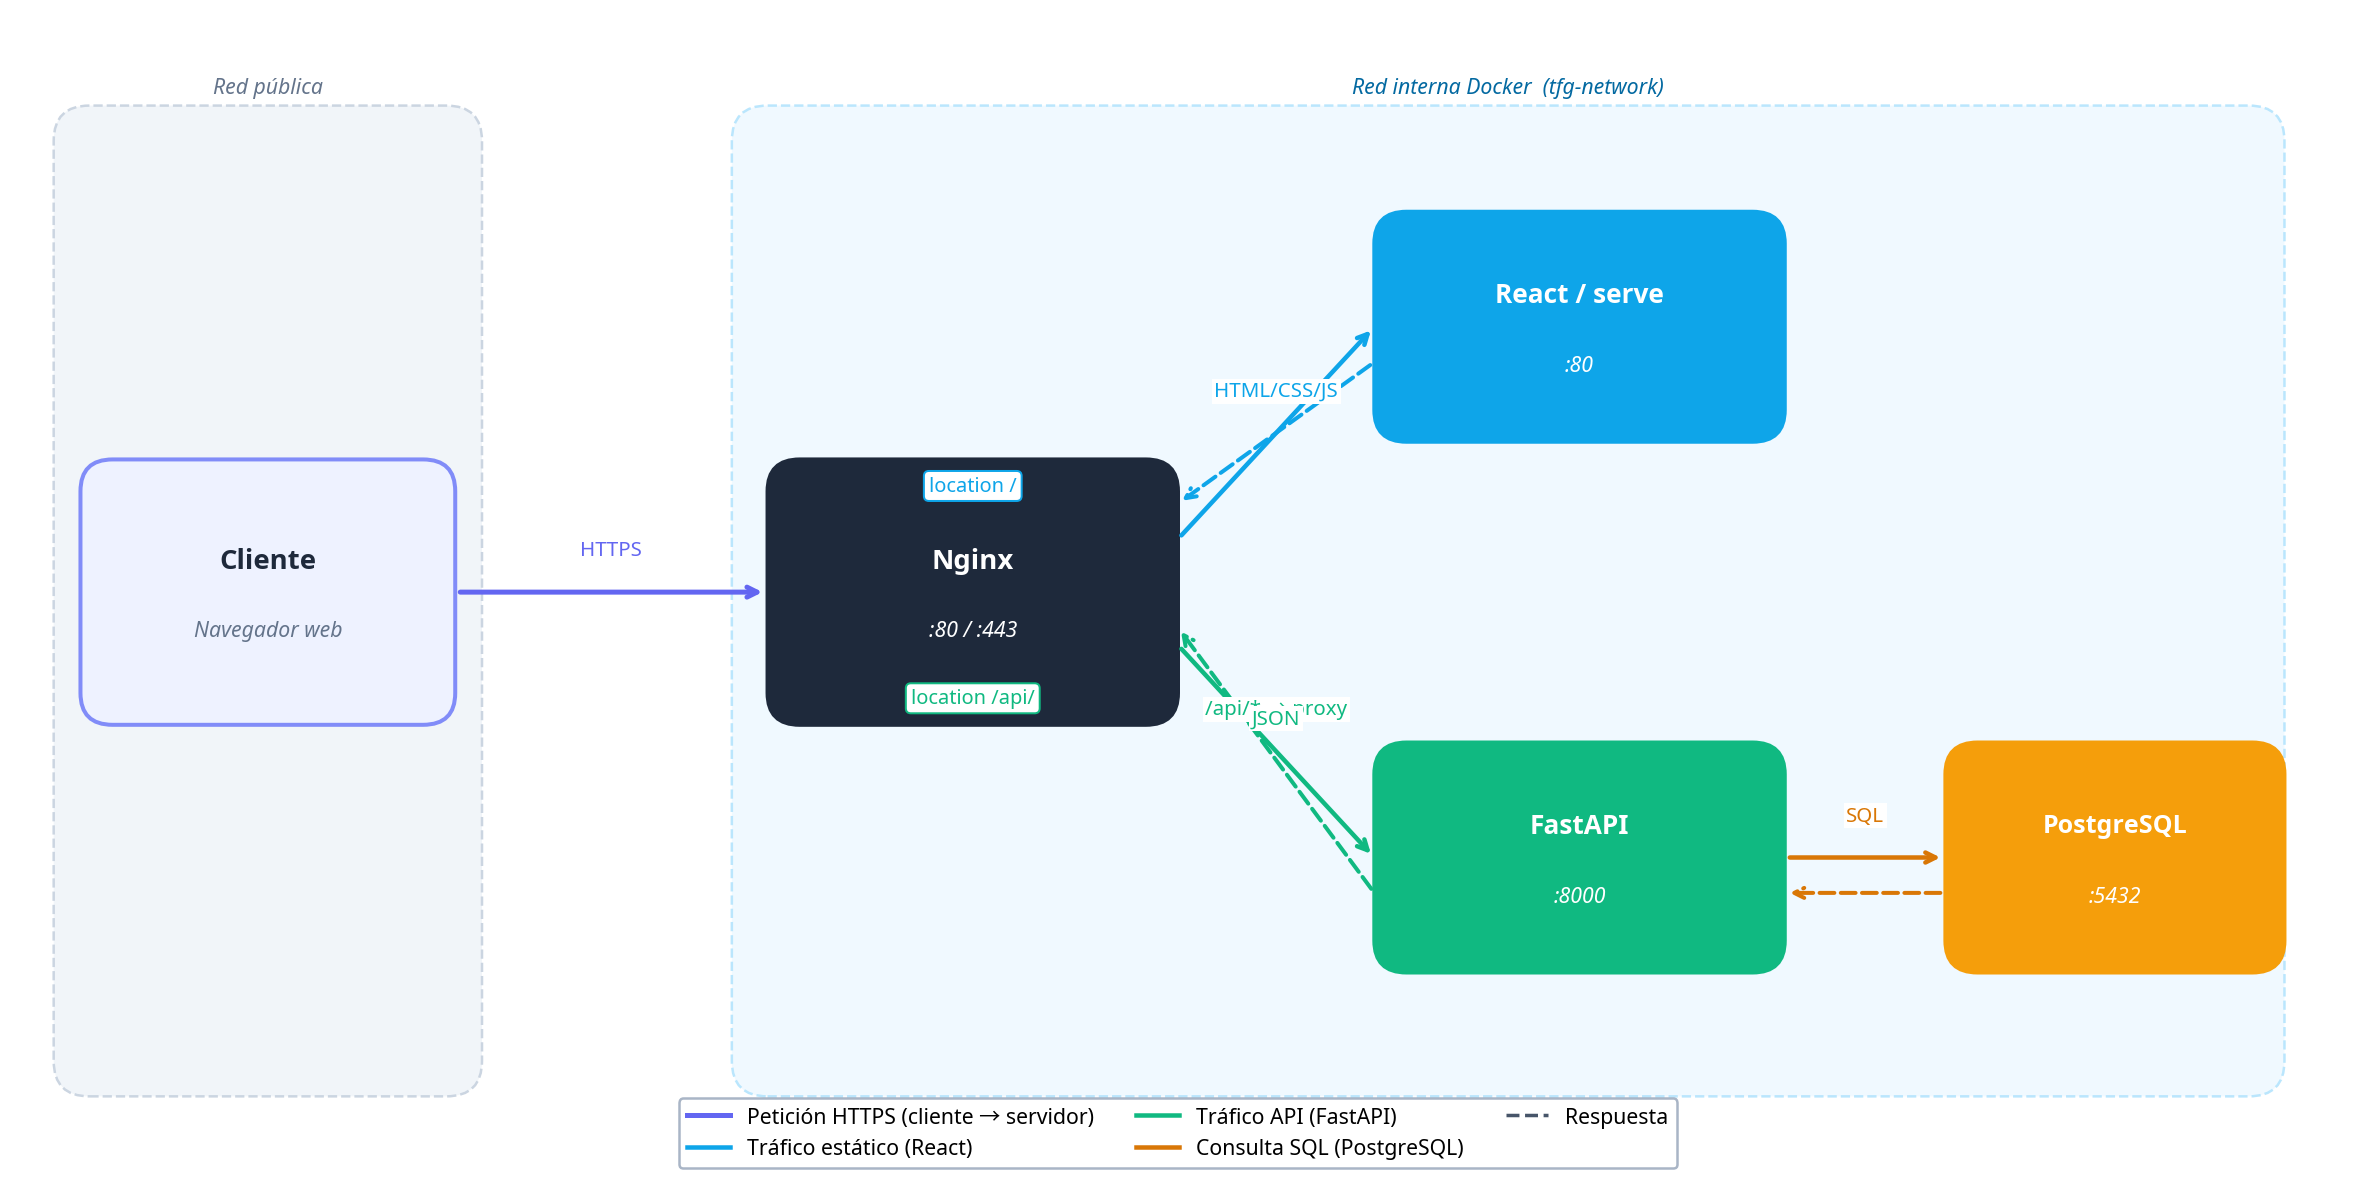
\includegraphics[width=0.85\textwidth]{imaxes/diagrama_nginx.png}
    \caption{Topología de despliegue y enrutamiento Nginx.}
    \label{fig:diagrama_nginx_deploy}
\end{figure}

% =========================================================================
\section{Backend RESTful (FastAPI)}
% =========================================================================

El backend se ha implementado con \textbf{FastAPI}~\cite{FastAPI_Docs} y SQLAlchemy~2.0. El contenedor arranca ejecutando migraciones Alembic, el \textit{seeding} del administrador y el servidor Uvicorn. 

La persistencia emplea un patrón dual sobre PostgreSQL: el esquema \textit{app} (lectura/escritura, gestionado por Alembic) alberga los usuarios, mientras que el esquema \textit{dwh} (solo lectura) mapea el Datamart (Figura~\ref{fig:diagrama_clases_backend}). La configuración sensible se inyecta mediante variables de entorno usando \textit{pydantic-settings}.

\subsection{Autenticación y roles}

La autenticación sigue el flujo JWT estándar (Figura~\ref{fig:jwt_flow}). Existen dos roles (\textit{admin} y \textit{viewer}), con reglas estrictas de protección sobre la cuenta del superadministrador (id=1), que no puede ser eliminada ni degradada.

\begin{figure}[htbp]
    \centering
    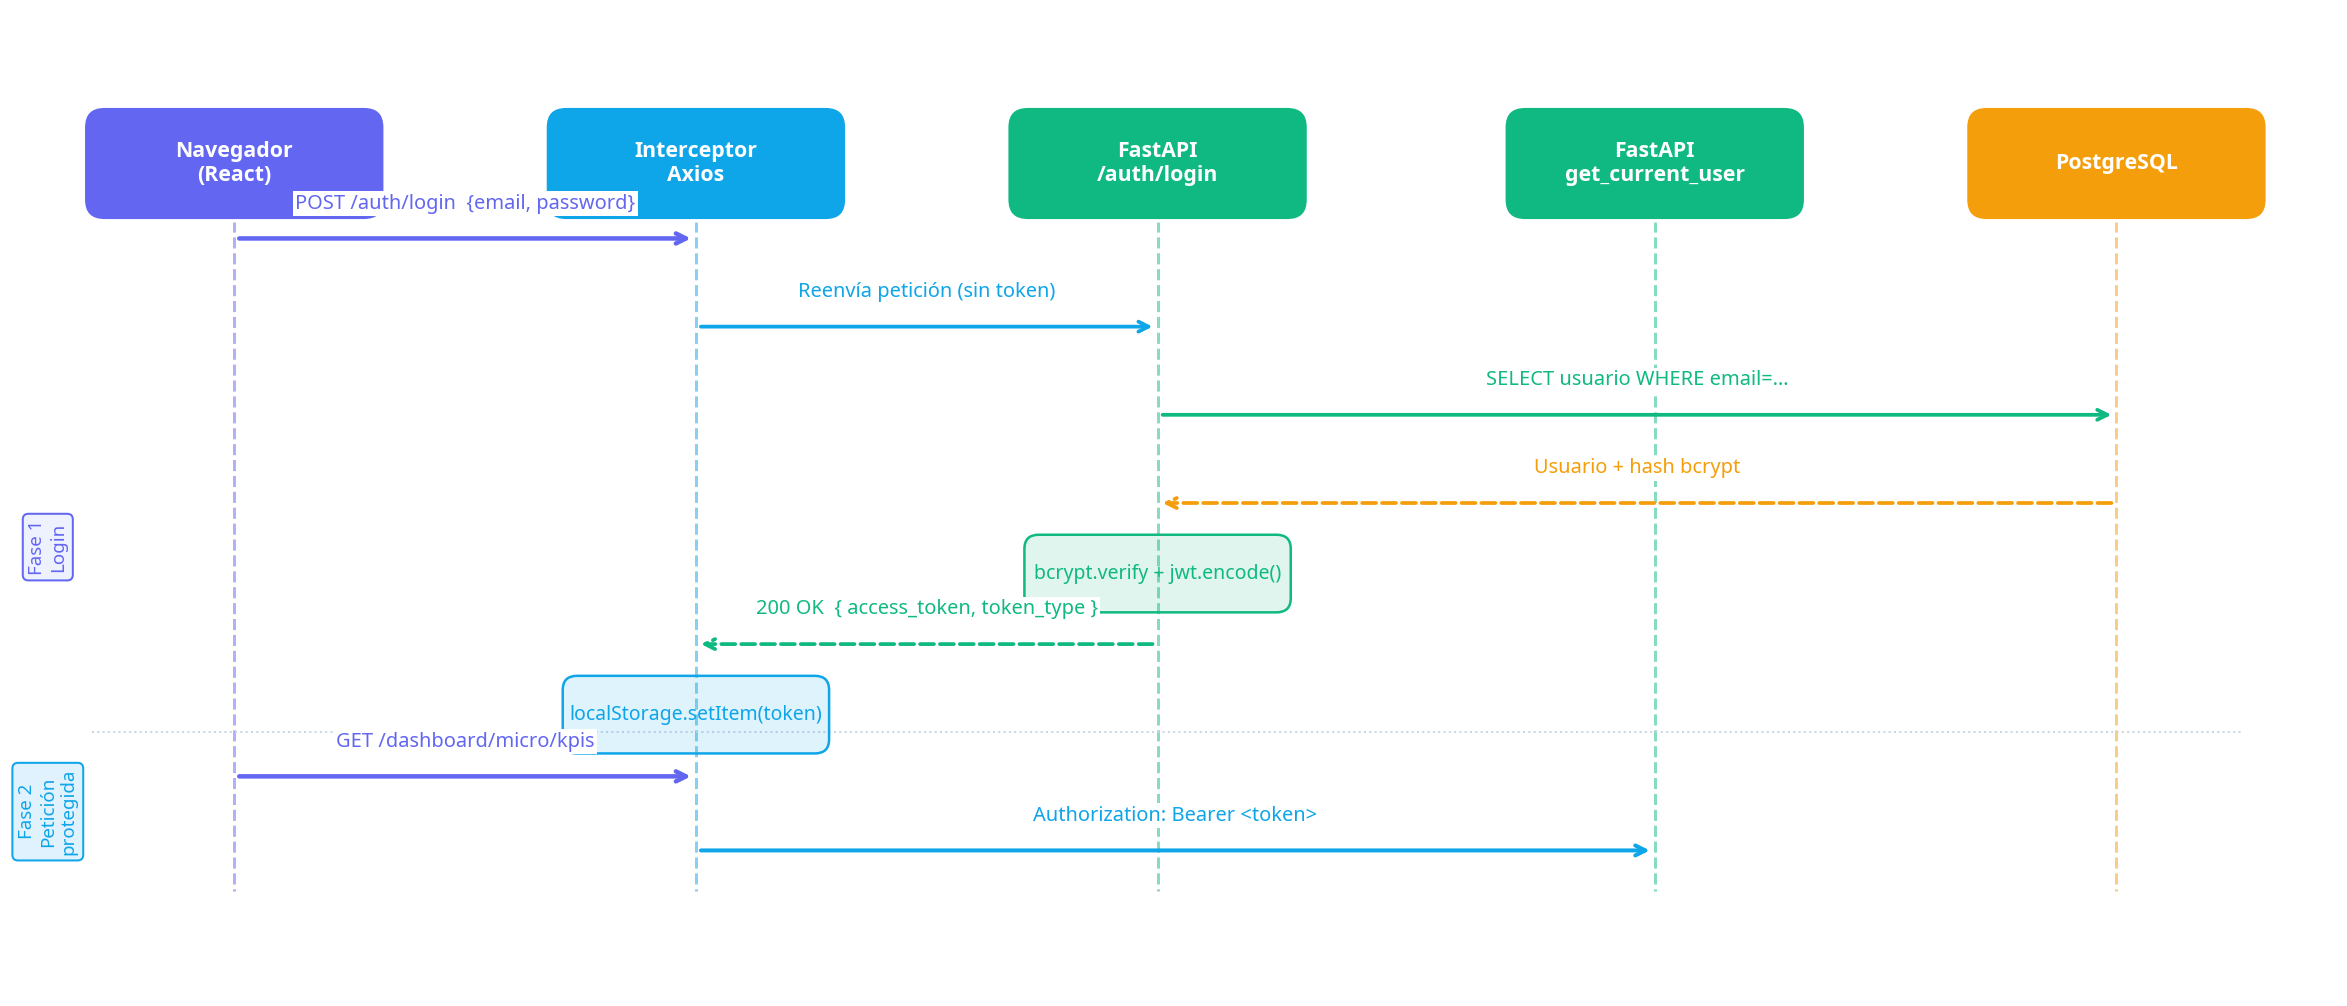
\includegraphics[width=0.85\textwidth]{imaxes/fig_jwt_flow.png}
    \caption{Flujo de autenticación JWT.}
    \label{fig:jwt_flow}
\end{figure}

\subsection{Arquitectura en capas}

El código del backend sigue una separación estricta de responsabilidades en cuatro capas, cuya organización se refleja en la Figura~\ref{fig:diagrama_clases_backend}:

\begin{itemize}
    \item \textbf{Routers} (\textit{app/routers/v1/}): Definen los endpoints HTTP, validan parámetros de entrada con \textit{Query} de FastAPI, inyectan las dependencias de autenticación y delegan en la capa CRUD.
    \item \textbf{Schemas} (\textit{app/schemas/}): Modelos Pydantic que definen la forma de las peticiones y respuestas JSON. Actúan como contrato tipado entre la API y el frontend, generando automáticamente la documentación OpenAPI.
    \item \textbf{CRUD} (\textit{app/crud/}): Contiene la lógica SQL y de negocio. \textit{crud\_dashboard.py} concentra todas las agregaciones analíticas; \textit{crud\_user.py} gestiona el ciclo de vida de usuarios.
    \item \textbf{Models} (\textit{app/models/}): Mapeo ORM de las tablas de los esquemas \textit{app} y \textit{dwh}.
\end{itemize}

El flujo de una petición autenticada al dashboard sigue la cadena: \textit{Router} $\rightarrow$ \textit{CRUD} $\rightarrow$ \textit{Session}/\textit{Model} $\rightarrow$ PostgreSQL.

\begin{figure}[htbp]
    \centering
    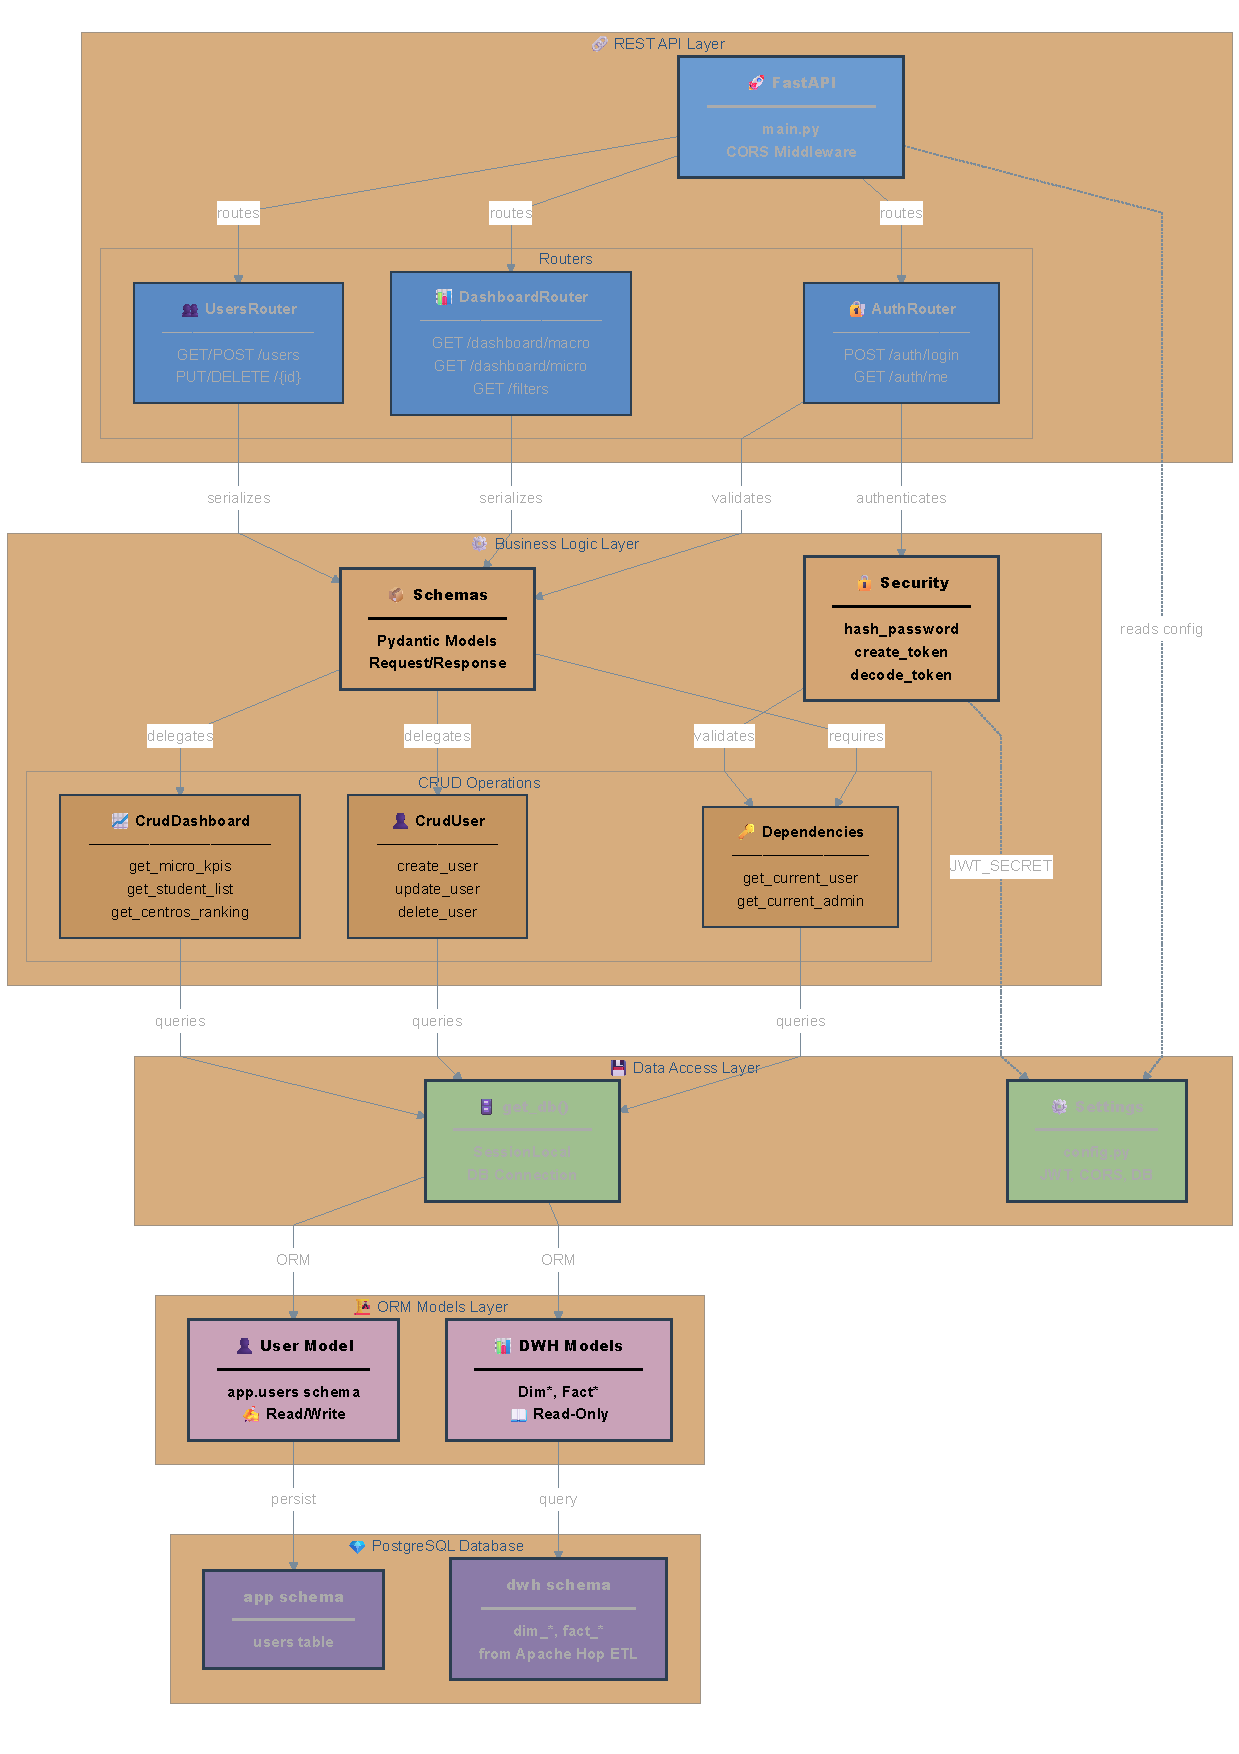
\includegraphics[width=0.9\textwidth]{imaxes/diagrama_backend.pdf}
    \caption{Diagrama de clases simplificado del backend FastAPI: interfaces REST, lógica de negocio y acceso a datos.}
    \label{fig:diagrama_clases_backend}
\end{figure}

\subsection{Motor de consultas analíticas}

Todas las consultas del dashboard parten de la función interna \textit{\_base\_query()}, que realiza un JOIN de \textit{fact\_rendimiento\_anual} con las seis dimensiones necesarias (Figura~\ref{fig:star_join}). Los identificadores de las claves foráneas en la tabla de hechos se castean a \textit{Integer} en los JOIN para compatibilizar tipos \textit{BigInteger} con las claves subrogadas de las dimensiones.

\begin{figure}[htbp]
    \centering
    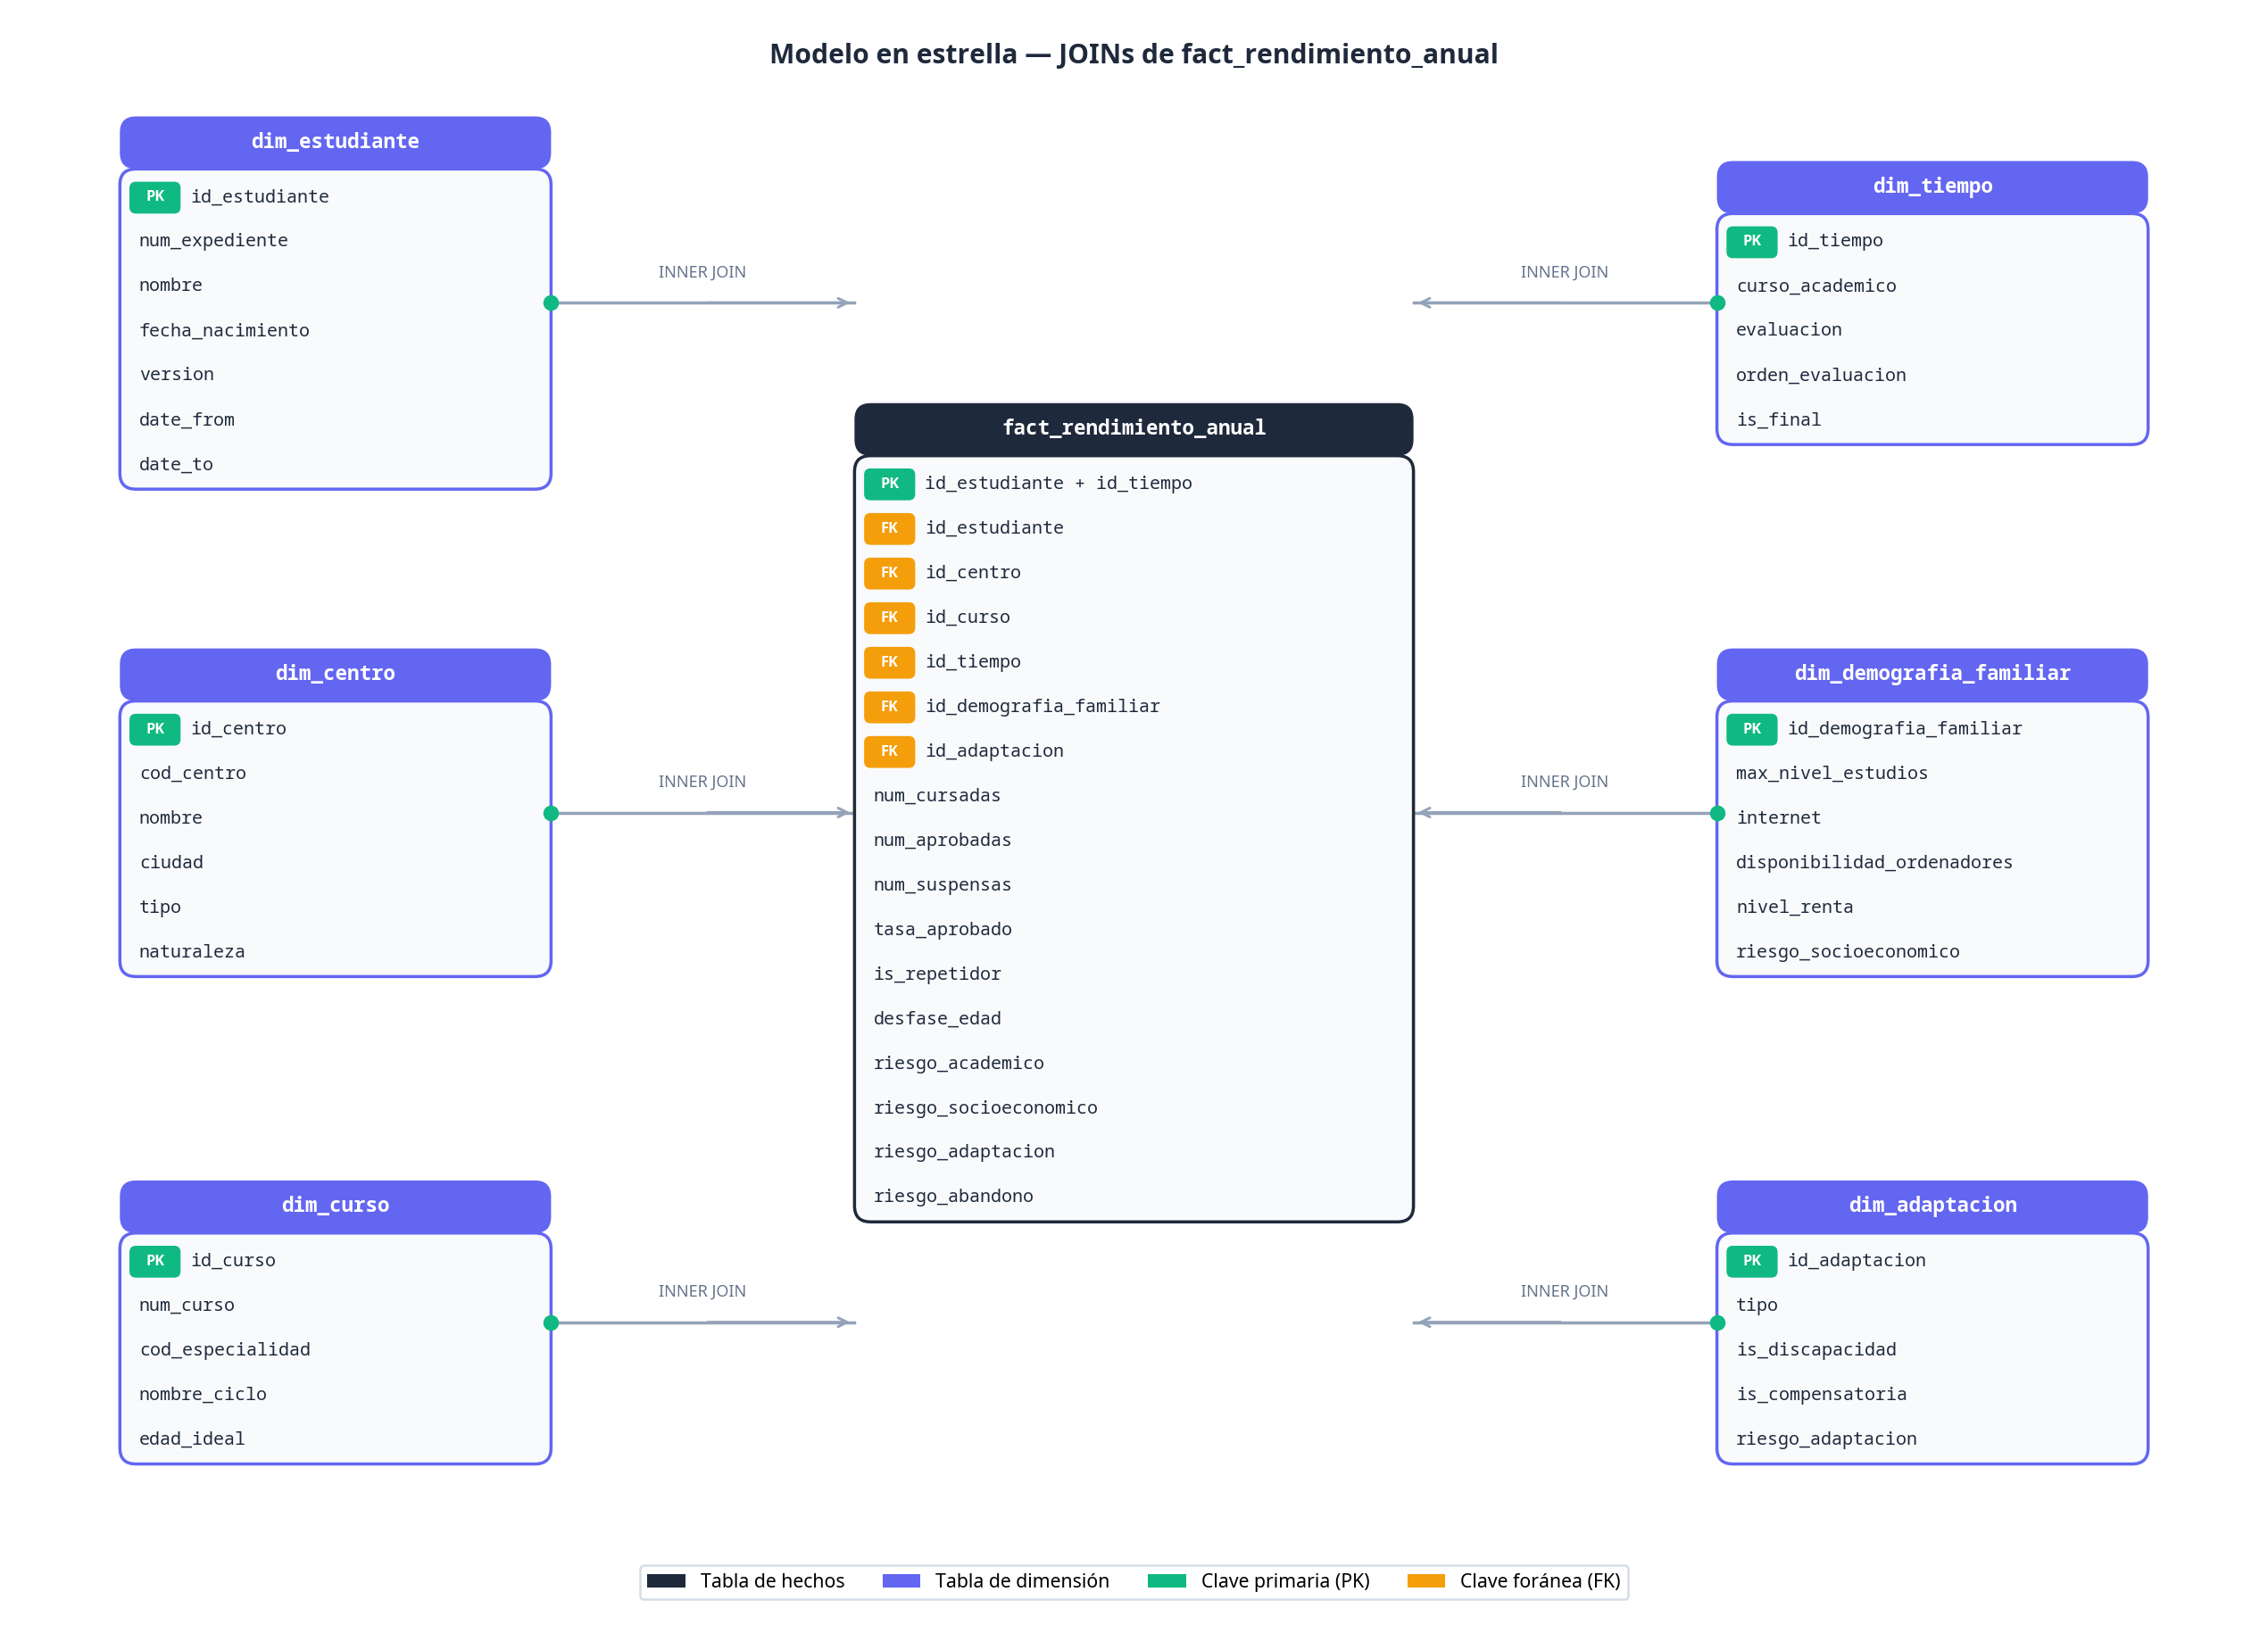
\includegraphics[width=0.85\textwidth]{imaxes/fig_star_join.png}
    \caption{Modelo en estrella base para consultas analíticas.}
    \label{fig:star_join}
\end{figure}

Sobre esta consulta base, la capa CRUD implementa las siguientes lógicas analíticas:

\begin{itemize}
    \item \textbf{Filtros dinámicos:} Permite selección múltiple en el frontend mediante parámetros de query repetidos (ej. \textit{?cod\_centro=A\&cod\_centro=B}) para filtrar por centro, curso, ciclo o tipo de centro.
    \item \textbf{Umbrales de riesgo proporcionales:} Calcula los umbrales de clasificación bajo, medio y alto a partir del máximo histórico de riesgo en el Datamart (25\% y 50\% del máximo respectivamente), evitando umbrales fijos que quedarían obsoletos si el ETL recalcula las ponderaciones.
    \item \textbf{Comparativa interanual (T0 vs T-1):} Si no se especifica curso, toma el más reciente. A partir de ese año (T0), calcula el curso anterior (T-1) y devuelve los contadores agrupados y aplanados con el sufijo \textit{\_a1} para facilitar la comparativa visual en el frontend.
    \item \textbf{Índice de riesgo por centro:} Agrega diez métricas de alerta por centro educativo (riesgo alto, repetidores, brecha digital, etc.) y calcula su porcentaje de incidencia. El índice de riesgo (0-10) es el número de métricas cuyo porcentaje supera la mediana autonómica.
    \item \textbf{Geocodificación:} Geocodifica cada centro mediante la librería \textit{geopy} (Nominatim de OpenStreetMap) usando el código postal y ciudad, cacheando las coordenadas en memoria para evitar llamadas repetidas a la API externa.
\end{itemize}

La Figura~\ref{tab:endpoints_dashboard} resume el catálogo de endpoints expuestos.

\begin{figure}[htbp]
    \centering
    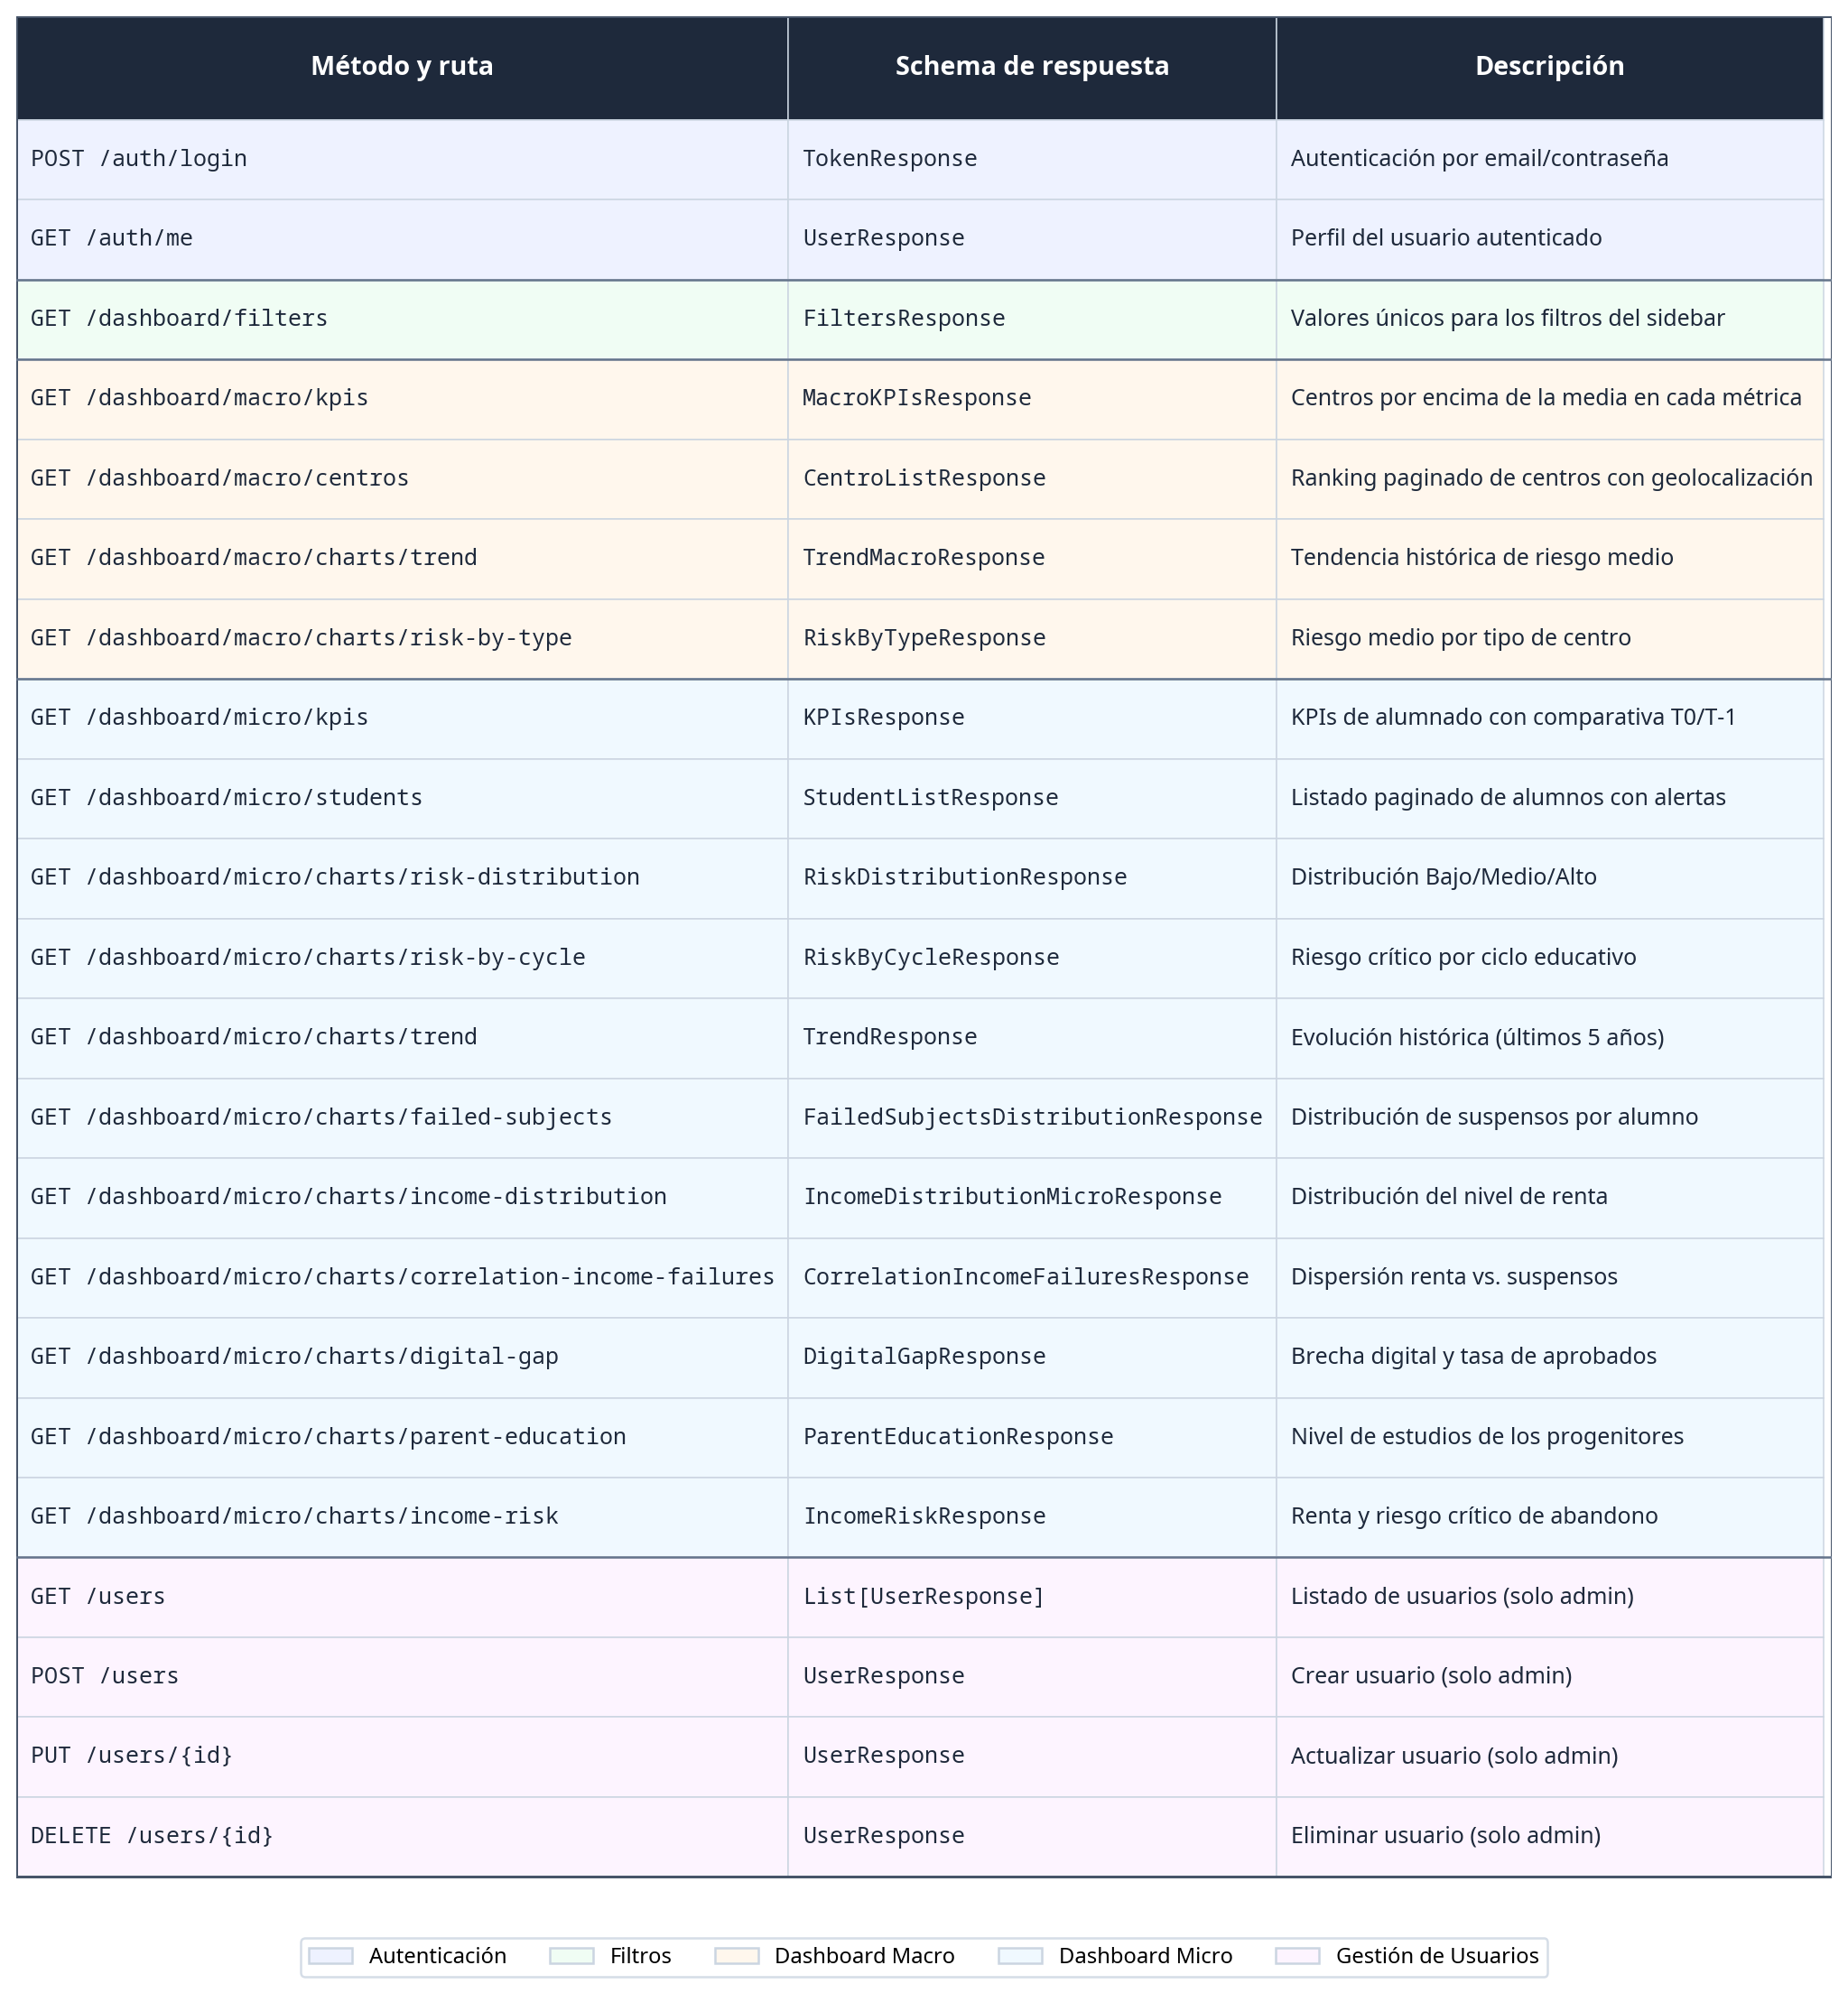
\includegraphics[width=0.85\textwidth]{imaxes/tabla_endpoints.png}
    \caption{Catálogo de endpoints de la API del dashboard (/api/v1).}
    \label{tab:endpoints_dashboard}
\end{figure}

% =========================================================================
\section{Frontend (React y Vite)}

La interfaz es una \textbf{Single Page Application (SPA)} desarrollada con React~18~\cite{React_Docs} y empaquetada con \textbf{Vite}~6. 

El Dockerfile implementa un build multi-etapa (Figura~\ref{fig:build_pipeline}): una etapa de compilación que genera los artefactos estáticos (\textit{npm run build}), y una etapa de producción basada en Node Alpine que sirve la aplicación mediante el paquete \textit{serve} en el puerto 80, delegando el \textit{fallback} de rutas a \textit{index.html}.

\begin{figure}[htbp]
    \centering
    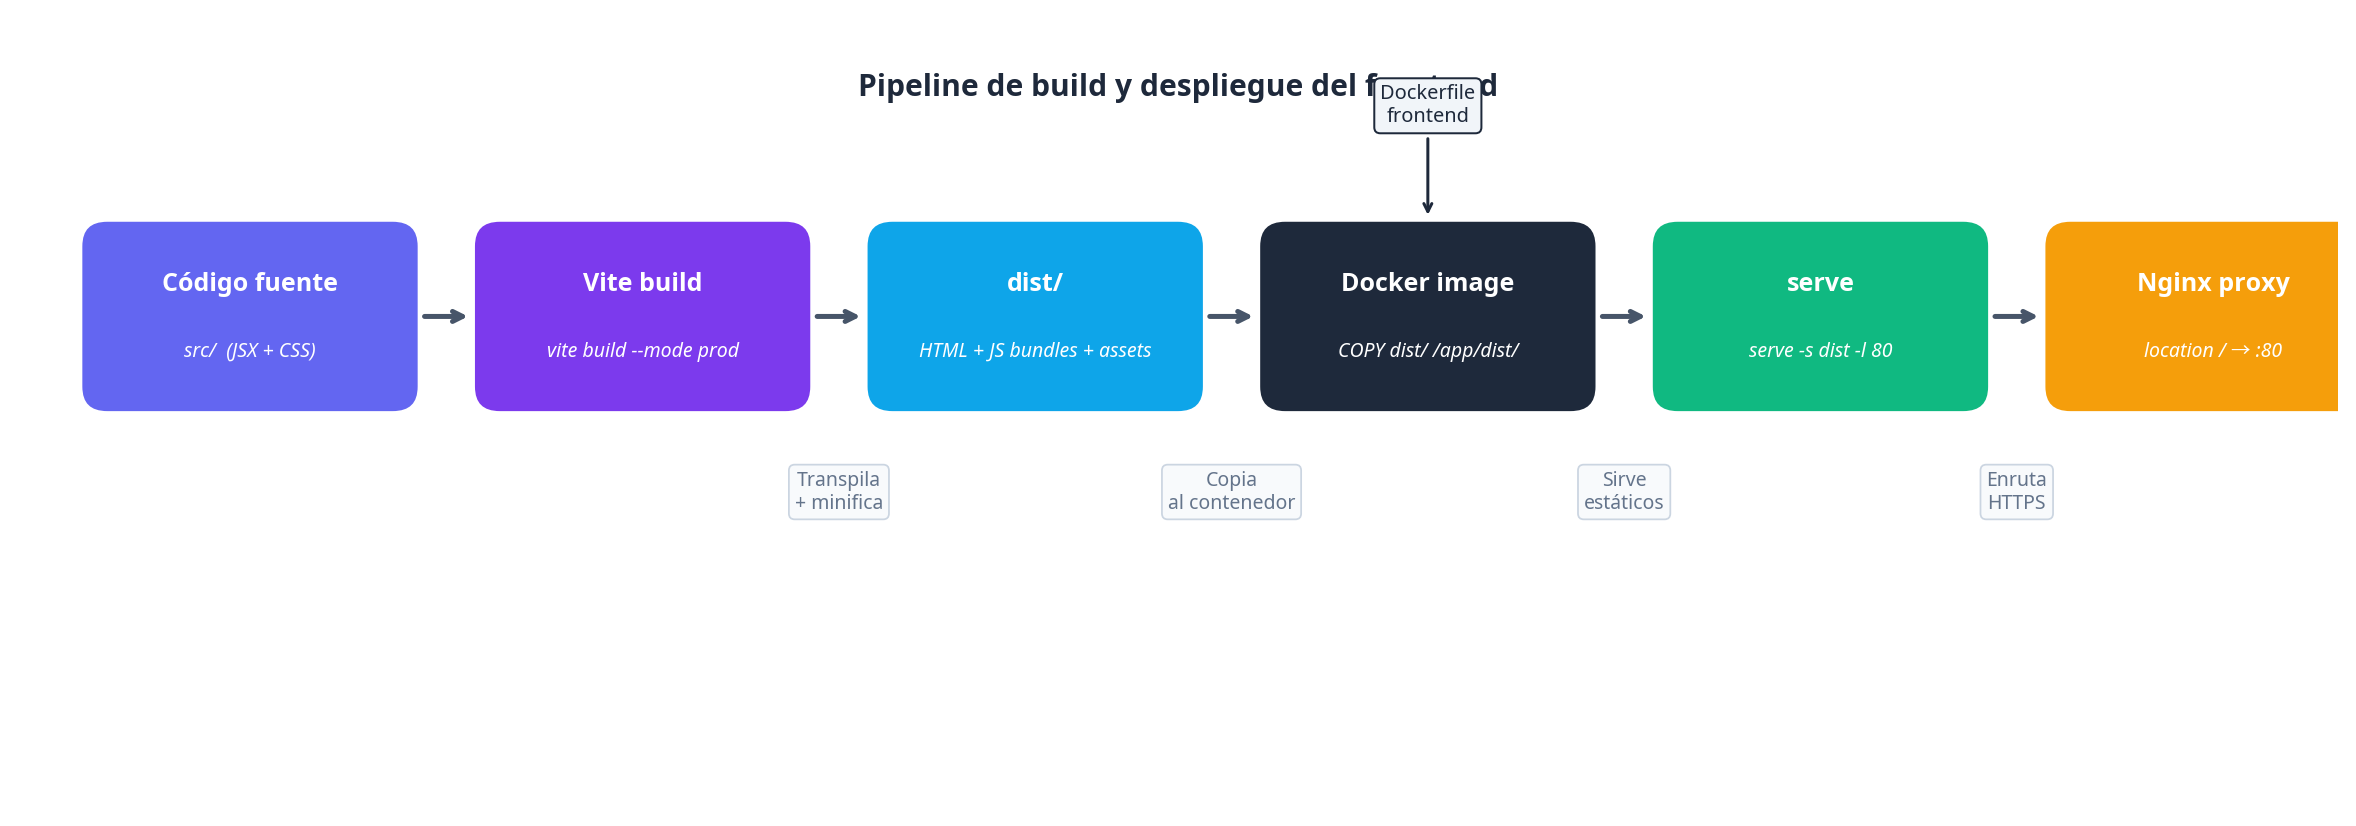
\includegraphics[width=0.85\textwidth]{imaxes/fig_build_pipeline.png}
    \caption{Pipeline de build y despliegue del frontend.}
    \label{fig:build_pipeline}
\end{figure}

Las dependencias clave incluyen \textbf{Axios} (cliente HTTP con interceptores JWT), \textbf{React Router} (enrutamiento), \textbf{Recharts} (gráficos D3), \textbf{Leaflet} (mapas) y \textbf{Lucide} (iconografía).

\subsection{Arquitectura del código fuente}

El directorio \textit{src/} se organiza en módulos técnicos (Figura~\ref{fig:frontend_tree}): \textbf{services} y \textbf{api} (instancia Axios y funciones de acceso al backend), \textbf{context} (estado global de autenticación y filtros), \textbf{pages} (vistas de la SPA) y \textbf{components} (UI reutilizable).

\begin{figure}[htbp]
    \centering
    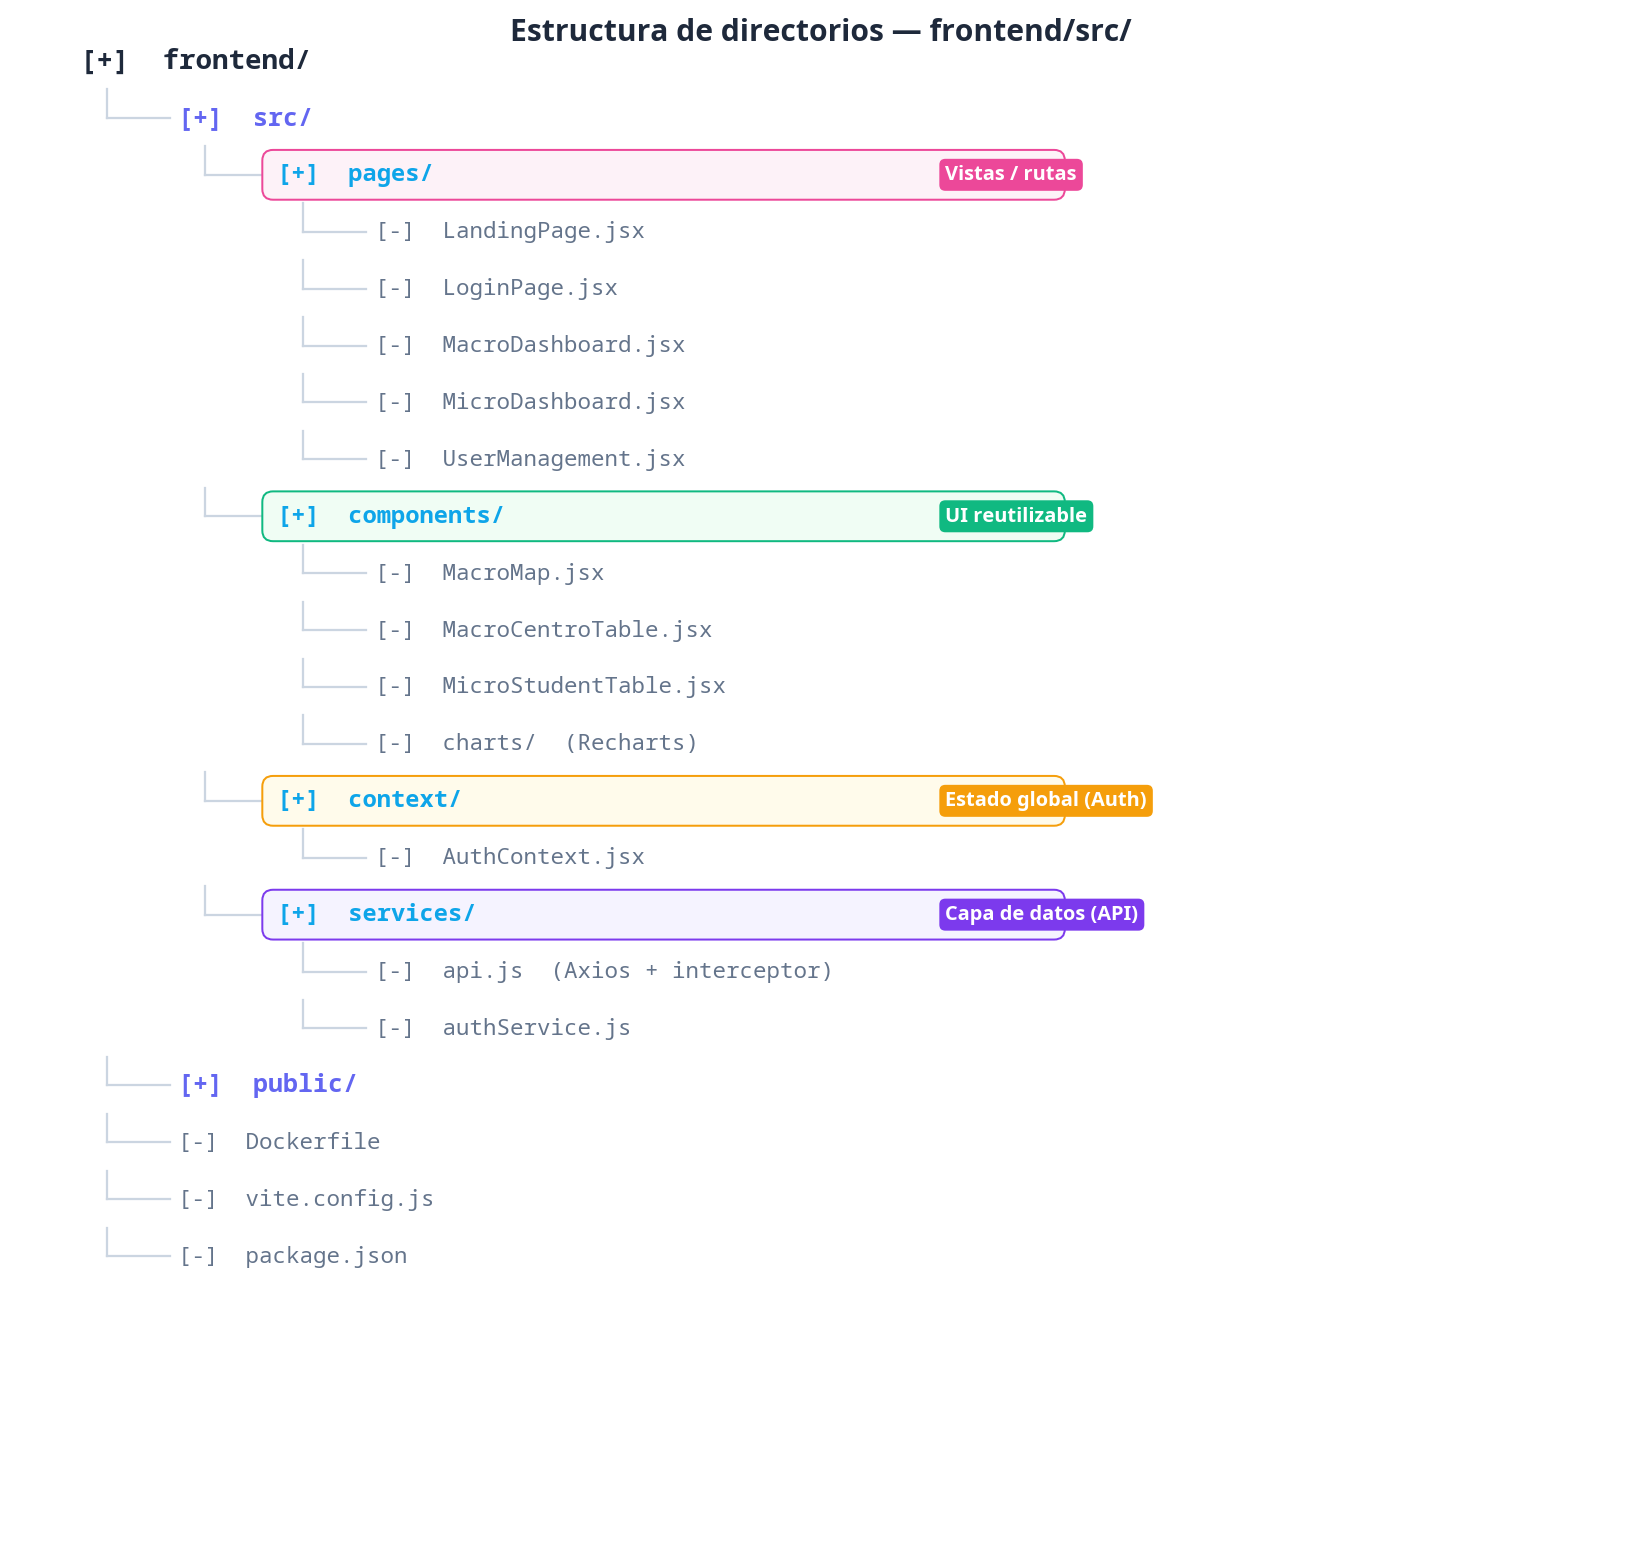
\includegraphics[width=0.6\textwidth]{imaxes/fig_frontend_tree.png}
    \caption{Estructura de directorios del frontend (src/).}
    \label{fig:frontend_tree}
\end{figure}

El enrutamiento (\textit{App.jsx}) protege las rutas \textit{/macro}, \textit{/micro} y \textit{/users} bajo un \textit{Layout} autenticado, redirigiendo a \textit{/login} si no hay token válido. El sistema de diseño prescinde de frameworks externos (Bootstrap, MUI), implementándose en CSS puro con variables nativas para soportar modo oscuro y una estética \textit{Glassmorphism} transversal a todos los componentes.

% =========================================================================
\section{Proxy inverso (Nginx)}

El contenedor \textit{nginx} es el único punto de entrada de la aplicación. Escucha en el puerto 80 para redirigir tráfico a HTTPS (puerto 443), donde termina el cifrado TLS con certificados montados en volumen.

Nginx define dos \textit{upstreams} internos de Docker (\textit{frontend} y \textit{api}) y enruta el tráfico basándose en la ruta solicitada (Figura~\ref{fig:nginx_routing}). Las peticiones al prefijo \textit{/api/} se reenvían al backend FastAPI (con \textit{timeouts} extendidos a 60 segundos para consultas analíticas pesadas), mientras que el resto de rutas y assets estáticos se proxifican al contenedor React. 

\begin{figure}[htbp]
    \centering
    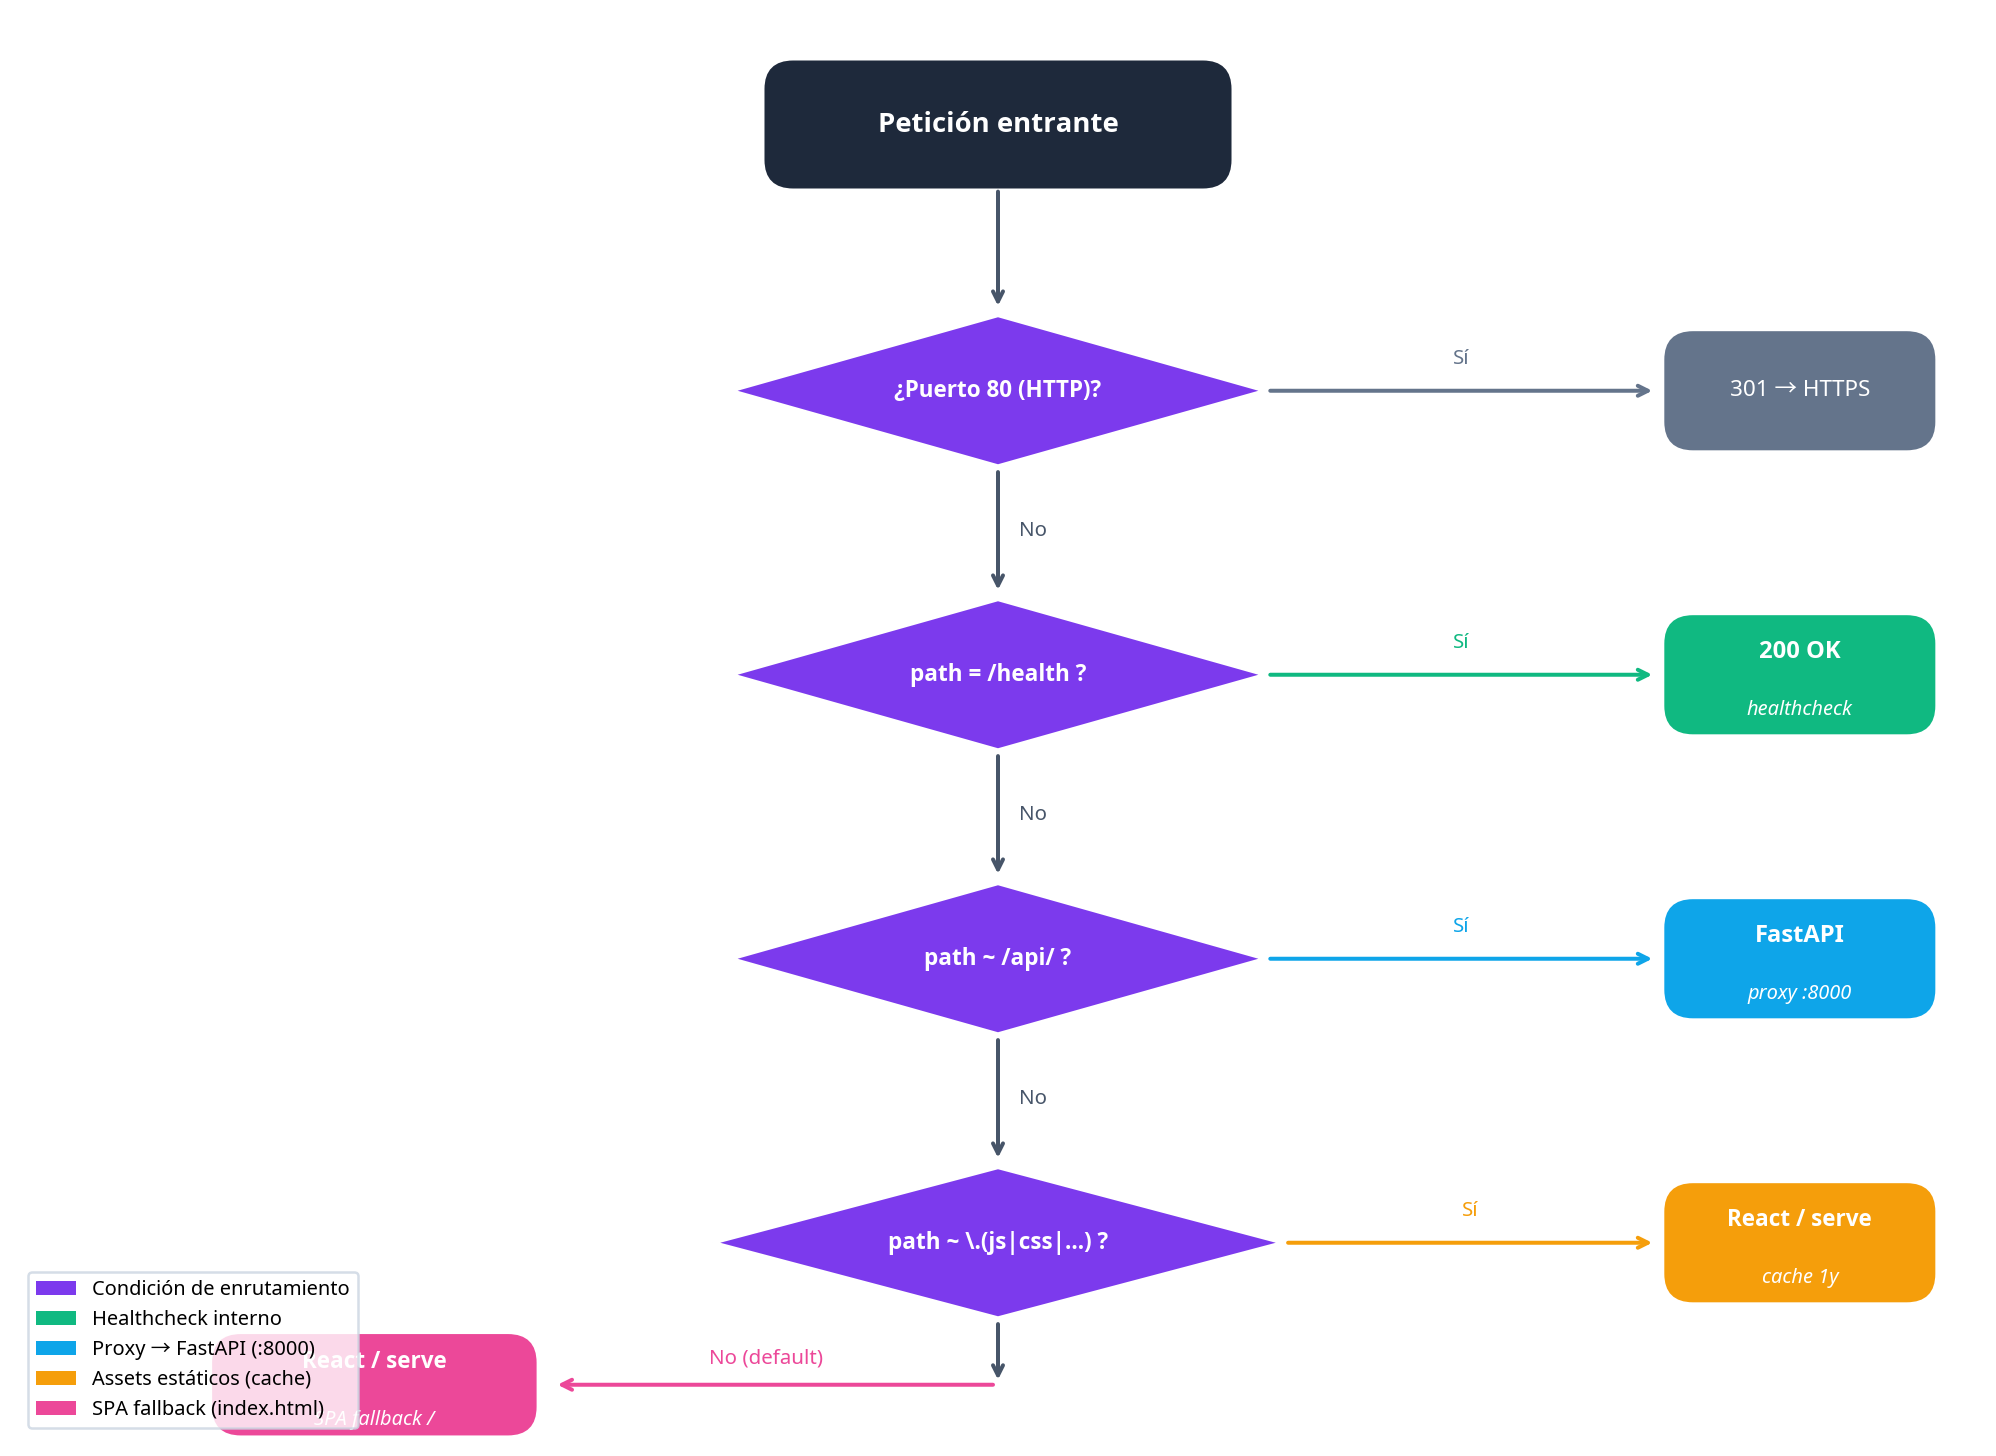
\includegraphics[width=0.72\textwidth]{imaxes/fig_nginx_routing.png}
    \caption{Diagrama de flujo de decisión del proxy inverso Nginx.}
    \label{fig:nginx_routing}
\end{figure}

Para optimizar el rendimiento, Nginx aplica compresión \textit{gzip} nivel 6 a respuestas JSON y assets estáticos, y añade cabeceras de caché de larga duración (1 año) para imágenes y fuentes tipográficas. Como resultado, ni la API, ni el frontend, ni las bases de datos exponen puertos directamente al \textit{host}, garantizando el aislamiento de la red interna.
